\section{Results}\label{sec:results}
Our framework applies to any activation function satisfying Assumption~\ref{assum:psi}, which covers B-splines (and hence deep-spline networks), Pad\'e approximations, Chebyshev polynomials, Gaussian processes, and Fourier-series activations, in addition to fixed activations such as tanh, sigmoid, and gelu. We perform our empirical evaluation on KAN networks~\cite{li2024kolmogorovarnold} specifically because each unit in a KAN carries its own independently learned activation function, unlike a standard feedforward network that reuses a single fixed nonlinearity (e.g., tanh or gelu) at every node. KANs use learnable representations at each node, meaning each activation function is  non-linear. Crucially, the functions differ across units and  thus a single abstraction for the entire network is not feasible.  This makes KANs a natural test for our method: every unit demands its own abstraction, and the choice of how to approximate each unit becomes a core decision problem rather than a one-time preprocessing step.

The KANs used in our analysis are trained using the FastKAN library~\cite{li2024kolmogorovarnold}.
%Their architecture closely resembles the original KAN implementation, it significantly accelerates training with a negligible performance tradeoff, as noted by the authors. 
Specifically, FastKAN replaces the B-spline basis functions of the original KAN with radial basis functions (RBFs), reducing computation time with negligible accuracy loss. Each activation function is a learned weighted sum of Gaussian RBFs, with the weights optimized independently per unit during training so each unit in the network carries a distinct nonlinear activation function. However, these functions satisfy Assumption~\ref{assum:psi}. As a linear combination of basis functions, we can compute bounds on the derivatives of the basis functions as linear combinations of bounds computed over the fixed basis functions. We use an initial interval analysis over the network to fix the domain of each activation function. 

\begin{figure*}[ht!]
    \centering
    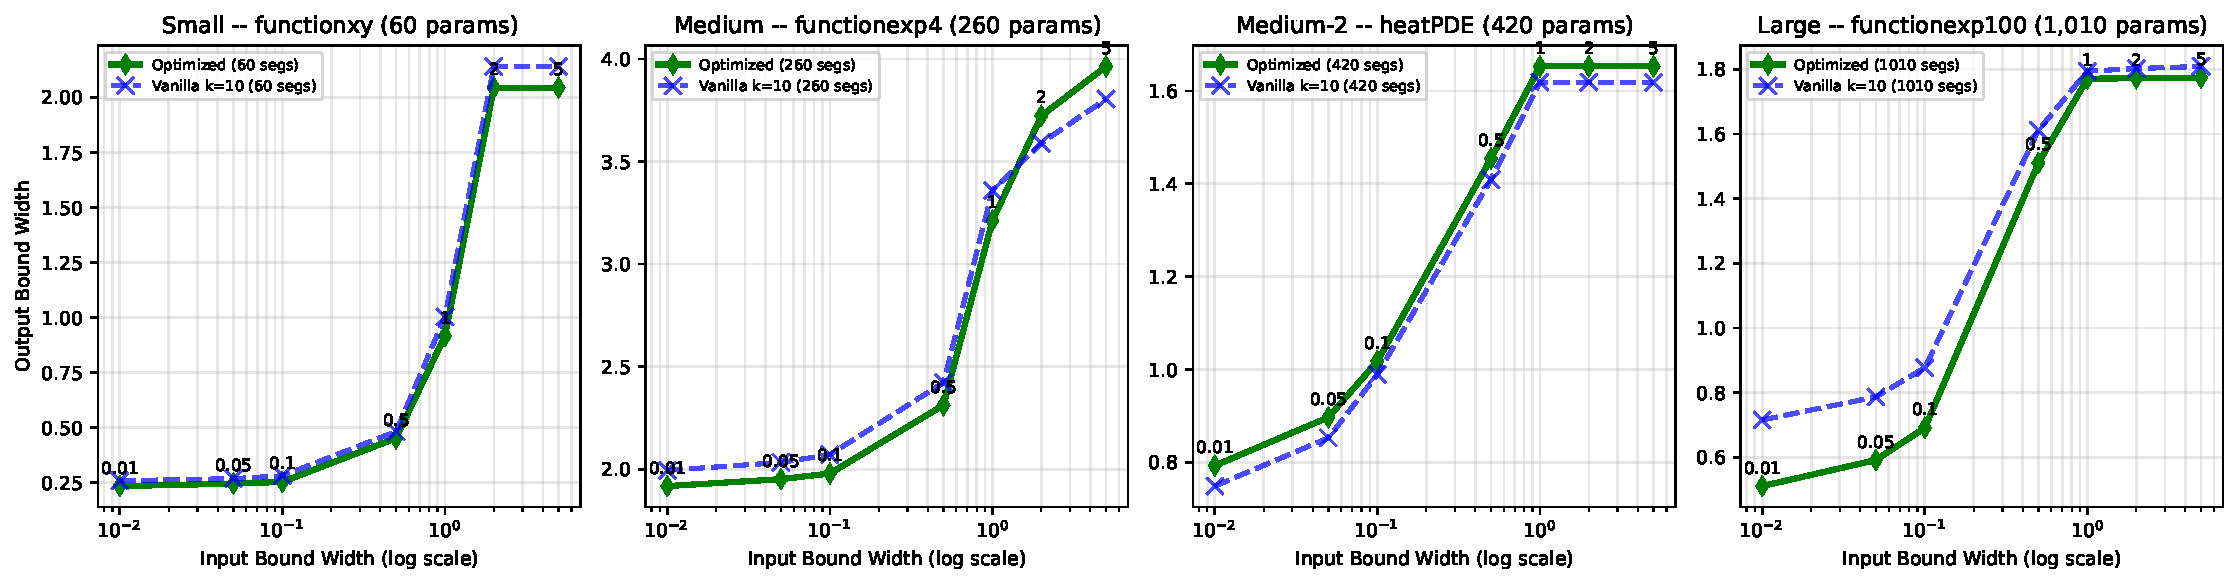
\includegraphics[width=1\linewidth, trim=5 5 5 5, clip]{images/plot_input_vs_output_width.pdf}
    \caption{Tightness of the methods compared by showing how the output bound width changes as input width is varied. We see that across all methods, the output bound width increases as the input bound width increases. \textcolor{red}{However, our method (\emph{Optimized}) consistently achieves tighter bounds than the baseline (\emph{Vanilla}) across all input widths.} \{Small: [2, 2, 1] KAN; Medium: [4, 4, 2, 1] KAN; Medium-2: [2, 10, 2, 1] KAN; Large: [100, 1, 1] KAN; (x params): x trainable parameters per KAN\}}\label{fig:iw_width}
\end{figure*}

The benchmarks are taken from a variety of sources including the KANs used for function approximations in the original paper~\cite{li2024kolmogorovarnold}, KANs trained on existing datasets and KAN model that solves differential equations such as the heat equation. 
In this paper we focus results on four models of various sizes. Further analyses for the main benchmarks and additional benchmarks are reported in Appendix~\ref{app:seg-width-main}, \ref{app:more-benchmarks}.

We run experiments on four types of KAN (\emph{Small}, \emph{Medium}, \emph{Medium-2}, and \emph{Large}) networks with increasing number of parameters. Note that number of parameters is an imperfect proxy for verification difficulty: the Large network ([100, 1, 1]) has a single hidden unit, whereas Medium-2 ([2, 10, 2, 1]) is deeper and produces a harder MILP despite having fewer parameters. Figure~\ref{fig:timing} reflects this: Medium-2 dominates verification time. We then compare the output tightness of our method (\emph{Optimized}) with the baseline (\emph{Vanilla}) approach. 

We consider two approaches: (a) \textbf{Vanilla}, the baseline method that uses a fixed number of segments $k$ for each unit and uses Bellman's algorithm to compute PWA at each node, and (b) \textbf{Optimized}, which solves a knapsack problem for total segment budget $B = k \cdot |\mathcal{S}|$ across splines by solving an ILP, where $|\mathcal{S}|$ is the total number of splines in the network.
\ck{For the Q2 timing comparison, both approaches use the same total number of pieces: uniformly for \textit{Vanilla}, and via the piece-budget-constrained ILP of Section~\ref{sec:optimalkan-abs} for \textit{Optimized}. The Q1 tightness comparison instead targets a fixed error budget, as described below.}

The \textit{Optimized} pipeline executes four stages for each verification. First, for each univariate activation function $\psi_{i,j}$, we run Bellman's DP to obtain a trade-off curve relating piece count to local error $e_{i,j}$. The DP table at each node is computed for the number of segments ranging from $1$ until $\max(S_{\max}, 2k)$, where $S_{\max} = 50$ is the default maximum; the $2k$ term ensures the table extends beyond the uniform budget when $k$ is large. \textit{Vanilla} simply uses a single fixed $k$ for all splines. Second, we estimate each activation function's Lipschitz constant to obtain  the sensitivity weights following the approach outlined in the proof of Theorem~\ref{thm:kan-overall-error}. \ck{Third, we encode the multi-choice knapsack as an integer program. For the input-width sweep, this program selects one row from each trade-off table to minimize total pieces used subject to a global error budget $\delta$ (the dual of the formulation in Section~\ref{sec:optimalkan-abs}, which instead fixes a piece budget and minimizes error). Both directions solve the same trade-off-table DP, just swapping which quantity is the objective and which is the constraint. We fix $\delta = 1.5 \cdot \delta_{\min}$, where $\delta_{\min} = \sum_s \min_k \tilde{e}_s(k)$ is the sum over splines of the minimum achievable Lipschitz-weighted approximation error. The $1.5\times$ slack gives the allocator room to trade error against pieces rather than pinning it to the best achievable error.} Fourth, with the abstraction now fixed, the chosen PWA abstraction is compiled into an MILP with the  MIP gap parameter of the solver set to $\epsilon_{\text{gap}} = 0.15$ and timeout $T = 500$. The \textit{Vanilla} approach using the uniform-$k$ abstraction also uses an MILP encoding to solve the verification problem. 

In our experiments we consider $\ell_\infty$-balls given by $\mathcal{B}_\infty(\mathbf{x}, r) = \{\mathbf{x}' \mid \|\mathbf{x} - \mathbf{x}'\|_\infty \leq r\}$ with radii $r \in \{0.01, 0.05, 0.1, 0.5, 1.0, 2.0, 5.0\}$ and we sweep segment counts $k \in \{1, 5, 10, 20, 30, 40, 50\}$. Our implementation is based on Python 3.11 and uses Gurobi as the MILP and ILP solver. All experiments are run with a fixed input domain centered at the origin and with fixed random seeds for reproducibility. \ck{We report a single run per benchmark rather than averaging over seeds, since the only randomness is in the initial network training and both the DP and ILP allocation steps are deterministic given a trained network. Timing numbers may still vary somewhat from run to run.}

\textbf{Overarching questions:}
We now describe the evaluation method on the benchmarks and ask the following two overarching questions: \emph{(1) does the Optimized approach yield tighter output bounds than the Vanilla baseline at equal segment budgets? what happens as the segment budget increases?} \emph{(2) does our approach scale as model parameters grow?}

\textbf{Learning tasks:} We consider four learning tasks: three special function approximation problems and one partial differential equation (PDE) solved using KANs. These examples are taken from the benchmarks of the original paper~\cite{Liu+Others/2025/KAN} and consist of four distinct learning scenarios. The tasks are:
\begin{enumerate}
    \item \emph{Small}: \texttt{funcxy}: $f(x, y) = x y$ (2 inputs; 60 parameters; [2, 2, 1] KAN)
    \item \emph{Medium}: \texttt{funcexp4}: $f(x_1, x_2, x_3, x_4) = \exp(\frac{1}{2}(\sin(\pi(x_1^2 - x_2^2)) + \sin(\pi(x_3^2 + x_4^2))))$ (4 inputs; 260 parameters; [4, 4, 2, 1] KAN)
    \item \emph{Medium-2}: \texttt{heatPDE}: $u_t = \nu u_{xx}$, $[x, t] \in [0,1] \times [0,1]$, $\nu = 0.01$ with Dirichlet boundary and sinusoidal initial conditions. (2 inputs; 420 parameters; [2, 10, 2, 1] KAN)
    \item \emph{Large}: \texttt{funcexp100}: $f(x_1,\dots,x_{100}) = \exp(\frac{1}{100}\sum_{i=1}^{100}\sin^2(\frac{\pi x_i}{2}))$ (100 inputs; 1010 parameters; [100, 1, 1] KAN)
\end{enumerate}
The sizes of the KANs are again determined by the best settings as reported in the original paper, and the training is done such that the models achieve a mean squared error (MSE) of less than $10^{-4}$ on a held-out test set.

\paragraph{\textbf{Q1: Bound Tightness --- Optimized vs.\ Uniform Allocation}}

\begin{figure*}[ht!]
    \centering
    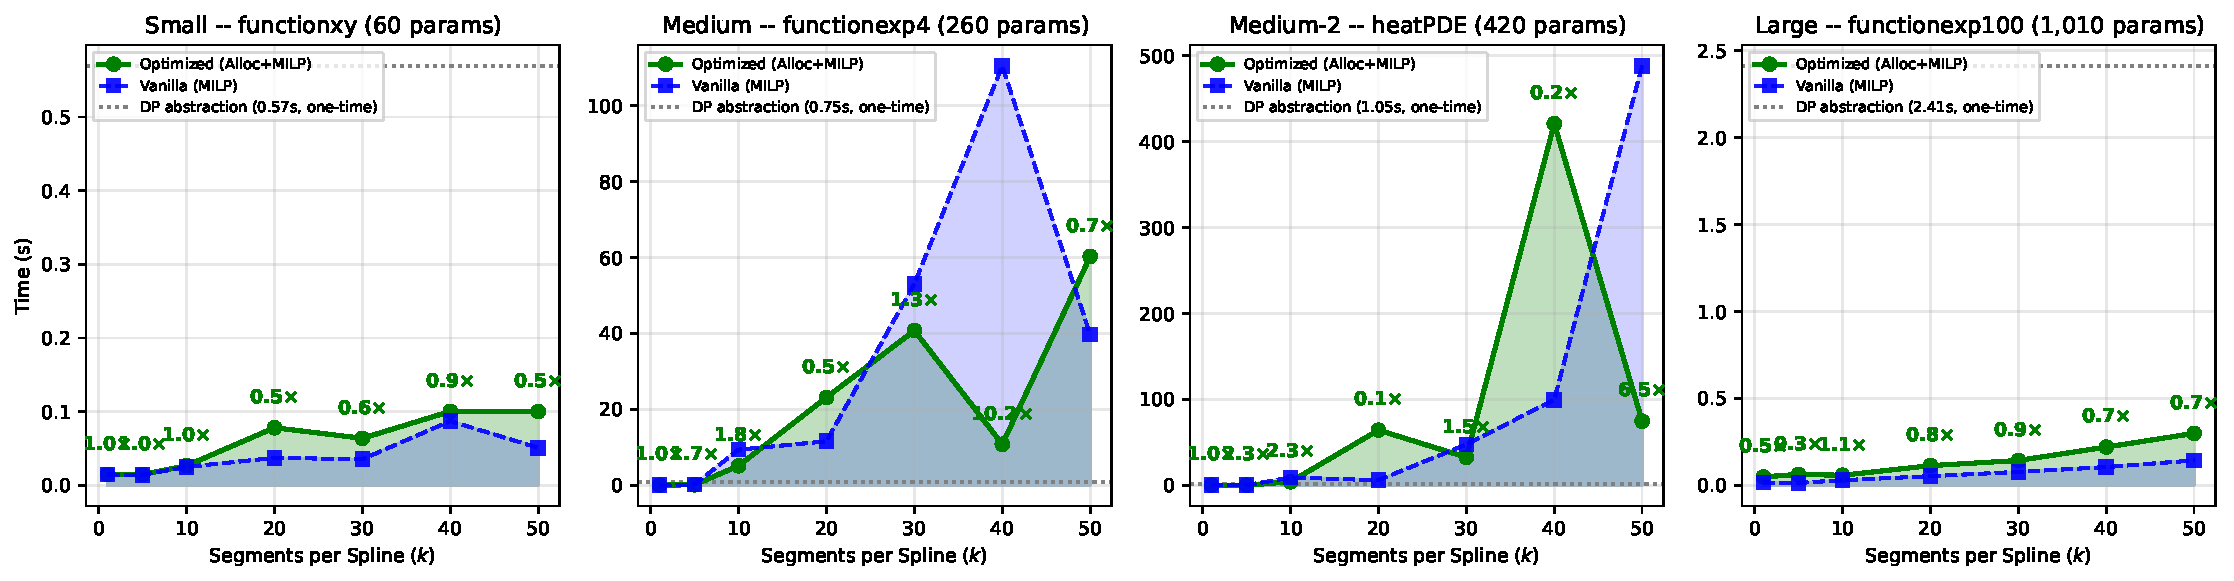
\includegraphics[width=1\linewidth, trim=5 5 5 5, clip]{images/plot_timing_summary.pdf}
        \caption{End-to-end runtime as a function of k. \textit{Optimized}'s per-query cost is the sum of the one-time DP abstraction (dotted line) and the downstream MILP (green); \textit{Vanilla} incurs only the MILP cost (dashed). \textcolor{red}{On Medium-2, where \textit{Vanilla}'s MILP scales sharply with k, \textit{Optimized} wins end-to-end at moderate-to-high k.} On Small and Large, \textit{Vanilla}'s MILP is already cheap and the DP overhead dominates single-query \textit{Optimized} runtime; the multipliers on the green curve show the MILP-stage runtime ratio (\textit{Vanilla} time / \textit{Optimized} time), which is the relevant quantity when the abstraction is amortized over multiple verification queries on the same network. A ratio above one indicates that \textit{Optimized}'s MILP stage is faster than \textit{Vanilla}'s at that budget; a ratio below one indicates the opposite. \{Small: [2, 2, 1] KAN; Medium: [4, 4, 2, 1] KAN; Medium-2: [2, 10, 2, 1] KAN; Large: [100, 1, 1] KAN; (x params): x trainable parameters per KAN\}}\label{fig:timing}
\end{figure*}


By varying the input perturbation radius and segment budget, we can evaluate the ablative tightness of the proposed method.  Figure~\ref{fig:iw_width} evaluates robustness under varying input perturbation radii. The advantage of optimized allocation is most pronounced in the small-radius regime, precisely where tight verification bounds are operationally most valuable. \textcolor{red}{For example, we see that the \emph{Small} benchmark at $r=0.01$ shows the optimized abstraction reduces the output width from $0.275$ to $0.025$, corresponding to an $11\times$ improvement. The gains are even larger on the \emph{Medium}, \emph{Medium-2}, and \emph{Large} networks, with the \emph{Large} benchmark reaching a $22\times$ improvement at $r=0.05$.} This behavior is consistent with the structure of interval error propagation i.e.~for small perturbation sets, approximation error accumulates primarily along a small number of highly sensitive spline paths, allowing the ILP allocator to concentrate segments where they maximally reduce propagated uncertainty, whereas uniform allocation expends budget indiscriminately across low-impact splines.

In contrast, as the perturbation radius increases, the verified bounds produced by both methods gradually tend to converge. In this regime, global nonlinear effects dominate local approximation error. \textcolor{red}{We also observe that, for the \emph{Large} benchmark at $r=0.01$, the optimized verifier returns $\infty$. In this case, the target approximation constraint $\delta = 1.5 \times \delta_{\min}$ is infeasible under the prescribed segment budget, indicating that there is no admissible PWA abstraction satisfying the target error without increasing $S_{\max}$.}

\textcolor{blue}{Noah: To assess how interval abstraction performs when applied as is, we replace the MILP with standard interval propagation through the uniform $k=10$ PWA abstraction. Table~\ref{tab:ibp-baseline} reports the resulting output widths alongside the MILP results of Fig.~\ref{fig:iw_width}. \textcolor{red}{With small radii, plain interval propagation is 3--12$\times$ looser than our optimized method, confirming the wrapping-effect coarseness noted in Section~\ref{sec:related}.} \textcolor{red}{Since the MILPs are solved to a 0.15 relative optimality gap, their reported bounds can sit marginally above the gap-free interval bounds over the same abstraction, as visible in the Vanilla column.}}

  \begin{table}[t]
    \caption{\textcolor{blue}{Noah: Mean verified output bound widths from plain interval bound
    propagation (IBP) through the uniform $k{=}10$ PWA abstraction, compared
    with the MILP-based \emph{Vanilla} and \emph{Optimized} results of
    Fig.~\ref{fig:iw_width}.}}
    \label{tab:ibp-baseline}
    \centering
    \begin{tabular}{llrrr}
    \hline
    Net & $r$ & IBP & Vanilla & Optimized \\
    \hline
    Small    & 0.01 & 0.260 & 0.259 & 0.235 \\
             & 0.1  & 0.283 & 0.282 & 0.254 \\
    \hline
    Medium   & 0.01 & 2.081 & 1.994 & 1.918 \\
             & 0.1  & 2.172 & 2.071 & 1.979 \\
    \hline
    Medium-2 & 0.01 & 0.752 & 0.748 & 0.792 \\
             & 0.1  & 1.009 & 0.989 & 1.018 \\
    \hline
    Large    & 0.01 & 0.715 & 0.715 & 0.511 \\
             & 0.1  & 0.877 & 0.877 & 0.691 \\
    \hline
    \end{tabular}
  \end{table}

\textcolor{blue}{Noah: A complementary allocation metric that is independent of the MILP solver: the number of pieces each method needs to certify the same weighted error bound $\delta = 1.5\,\delta_{\min}$. Across all four benchmarks the optimized allocation needs $8$--$22\%$ fewer pieces than the best uniform choice of $k$ (Table~\ref{tab:eqerror}).}

  \begin{table}[t]
    \caption{\textcolor{blue}{Noah: Pieces required to certify the same weighted error bound $\delta = 1.5\,\delta_{\min}$: optimized allocation versus the smallest uniform $k$ meeting $\delta$.}}
    \label{tab:eqerror}
    \centering
    \textcolor{blue}{
    \begin{tabular}{lrrr}
    \hline
    Net & Optimized & Uniform & Savings \\
    \hline
    Small    & 182 & 198 ($k=33$) & 8\% \\
    Medium   & 873 & 1{,}014 ($k=39$) & 14\% \\
    Medium-2 & 1{,}177 & 1{,}512 ($k=36$) & 22\% \\
    Large    & 3{,}220 & 3{,}636 ($k=36$) & 11\% \\
    \hline
    \end{tabular}}
  \end{table}

%% DO NOT call out figures in appendices from within the ppaer.
%Figure~\ref{fig:seg_width} (Appendix~\ref{app:seg-width-main}) further reports the verified output bound width as a function of the segment budget $k$, where \emph{Vanilla} assigns $k$ segments uniformly to every spline and \emph{Optimized} allocates the equivalent global budget $B = k \cdot |\mathcal{S}|$ through the ILP formulation.

\paragraph{\textbf{Q2: Computation Time Comparison}}

Figure~\ref{fig:timing} reports end-to-end verification time as a function of the segment budget. \textcolor{red}{The one-time dynamic-programming abstraction overhead is modest: $0.15$s, $0.43$s, $1.01$s, and $1.82$s for the networks respectively.} This preprocessing phase parallelizes across splines, so its cost grows slowly with model size relative to the MILP stage. Consequently, the abstraction overhead becomes negligible when amortized across multiple verification queries. This is important because a single abstraction of the network can be reused across an unlimited number of verification queries such as varying input radius, target output property, or input feature for sensitivity analysis without re-running the DP. In practice, neural network certification pipelines issue many such queries per model~\cite{SinghEtAl2019AbstractDomain}, so the upfront abstraction cost is amortized over the entire query set, not charged per query.

\textcolor{red}{For the \emph{Small} benchmark, the optimized verifier achieves a consistent $1.6$--$3.3\times$ MILP runtime improvement over uniform allocation across all budgets. The speedup originates from the sparsity induced by adaptive allocation: low-sensitivity splines receive few breakpoints, substantially reducing the size of the downstream MILP encoding. The effect becomes significantly more pronounced on the \emph{Large} benchmark ($100$ inputs, $1010$ parameters). At $k = 50$, the optimized verifier's MILP solves in $0.09$s compared to $1.46$s for the uniform baseline, a  $15.1\times$ reduction in solver time. When the one-time DP abstraction cost of $1.82$s is included, this overhead is recovered after approximately two verification queries.}


This constitutes the principal scalability result of the framework. Under uniform allocation, the MILP formulation grows proportionally to $|\mathcal{S}| \times k$, yielding up to $5000$ PWA breakpoints for the \emph{Large} benchmark at $k=50$. Such uniformly dense encodings substantially increase branch-and-bound complexity and weaken solver pruning efficiency. In contrast, the optimized formulation concentrates representational complexity only along verification-critical spline regions.
The \emph{Medium} and \emph{Medium-2} benchmarks again exhibit non-monotone behavior, with runtime ratios varying as expected. This suggests that minimizing propagated approximation error alone is insufficient as an allocation objective and motivates future formulations to derive better ways to predict the complexity of MILPs generated from the PWA abstractions.
